
\documentclass{article}


\usepackage{amsmath,amsfonts,amsthm,amssymb,amsopn,bm}
% \usepackage{fullpage}
\usepackage[margin=.9in]{geometry}
\usepackage{graphicx}
% \usepackage{fullpage}
% \usepackage[paper=letterpaper,margin=1in,includeheadfoot,footskip=0.25in,headsep=0.25in]{geometry}
\usepackage{url}
\usepackage[usenames,dvipsnames]{color}
% \usepackage[pdfborder={0 0 1},colorlinks=true,citecolor=black,plainpages=false]{hyperref}
\usepackage{fancyhdr}
\usepackage{listings}
%\usepackage[ruled]{algorithm2e}
%\usepackage{multirow}
\newcommand{\field}[1]{\mathbb{#1}}
\newcommand{\1}{\mathbf{1}}
% \newcommand{\E}{\mathbb{E}} % real domain
\renewcommand{\P}{\mathbb{P}} % real domain
% \newcommand{\R}{\field{R}} % real domain
% \newcommand{\C}{\field{C}} % complex domain
\newcommand{\F}{\field{F}} % functional domain

\newcommand{\T}{^{\textrm T}} % transpose


\def\diag{\text{diag}}

%% operator in linear algebra, functional analysis
\newcommand{\inner}[2]{#1\cdot #2}
\newcommand{\norm}[1]{\left\|#1\right\|}
\newcommand{\twonorm}[1]{\|#1\|_2^2}
% operator in functios, maps such as M: domain1 --> domain 2
\newcommand{\Map}[1]{\mathcal{#1}}
\renewcommand{\theenumi}{\alph{enumi}} 

\newcommand{\Perp}{\perp \! \! \! \perp}

\def\E{\mathbb{E}}
\def\P{\mathbb{P}}
\def\R{\mathbb{R}}
\newcommand{\mb}[1]{\mathbf{#1}}
\newcommand{\mc}[1]{\mathcal{#1}}


\newcommand\independent{\protect\mathpalette{\protect\independenT}{\perp}}
\def\independenT#1#2{\mathrel{\rlap{$#1#2$}\mkern2mu{#1#2}}}
\newcommand{\vct}[1]{\boldsymbol{#1}} % vector
\newcommand{\mat}[1]{\boldsymbol{#1}} % matrix
\newcommand{\cst}[1]{\mathsf{#1}} % constant
\newcommand{\ProbOpr}[1]{\mathbb{#1}}
\newcommand{\grade}[1]{\small\textcolor{magenta}{\emph{[#1 points]}} \normalsize}
\date{{}}
%\graphicspath{ {./temp_img} }
\setlength\parindent{0px}

\begin{document}
\title{Homework \#1}
\author{\normalsize{CSE 546: Machine Learning}\\
\normalsize{Michael Ross}}
\maketitle


\section{Gaussians}
Recall that for any vector $u \in \R^n$ we have $||u||_2^2 = u^T u = \sum_{i=1}^n u_i^2$ and $||u||_1 = \sum_{i=1}^n |u_i|$. 
For a matrix $A \in \R^{n \times n}$ we denote $|A|$ as the determinant of $A$.
A multivariate Gaussian with mean $\mu \in \R^n$ and covariance $\Sigma \in \R^{n \times n}$ has a probability density function $p(x| \mu, \Sigma) =  \frac{1}{\sqrt{(2\pi)^n |\Sigma|}} \exp( -\frac{1}{2} (x-\mu)^T \Sigma^{-1} (x-\mu) )$ which we denote as $\mathcal{N}(\mu,\Sigma)$. \\

1. \grade{4} Let 
\begin{itemize}
\item $\mu_1 = \begin{bmatrix} 1 \\ 2 \end{bmatrix}$ and $\Sigma_1 = \begin{bmatrix} 1 & 0 \\ 0 & 2 \end{bmatrix}$
\item $\mu_2 = \begin{bmatrix} -1 \\ 1 \end{bmatrix}$ and $\Sigma_2 = \begin{bmatrix} 2 & -1.8 \\ -1.8 & 2 \end{bmatrix}$
\item $\mu_3 = \begin{bmatrix} 2 \\ -2 \end{bmatrix}$ and $\Sigma_3 = \begin{bmatrix} 3 & 1 \\ 1 & 2 \end{bmatrix}$
\end{itemize}
For each $i=1,2,3$ on a separate plot:
\begin{enumerate}
  \item Draw $n=100$ points $X_{i,1},\dots,X_{i,n} \sim \mathcal{N}(\mu_i, \Sigma_i)$ and plot the points as a scatter plot with each point as a triangle marker (Hint: use \texttt{numpy.random.randn} to generate a mean-zero independent Gaussian vector, then use the properties of Gaussians to generate $X$).
  \item Compute the sample mean and covariance matrices $\widehat{\mu}_i = \frac{1}{n} \sum_{j=1}^n X_{i,j}$ and $\widehat{\Sigma}_i = \frac{1}{n-1} \sum_{j=1}^n (X_{i,j} - \widehat{\mu}_i)^2$. 
  Compute the eigenvectors of $\widehat{\Sigma}_i$. Plot the eigenvectors as line segments originating from $\widehat{\mu}_i$ and have magnitude equal to the square root of their corresponding eigenvalues.
  \item If $(u_{i,1},\lambda_{i,1})$ and $(u_{i,2},\lambda_{i,2})$ are the eigenvector-eigenvalue pairs of the sample covariance matrix with $\lambda_{i,1} \geq \lambda_{i,2}$ and $||u_{i,1}||_2 = ||u_{i,2}||_2 = 1$, for $j=1,\dots,n$ let $\widetilde{X}_{i,j} = \begin{bmatrix} \frac{1}{\sqrt{\lambda_{i,1}}} u_{i,1}^T (X_{i,j} - \widehat{\mu}_i) \\ \frac{1}{\sqrt{\lambda_{i,2}}} u_{i,2}^T (X_{i,j} - \widehat{\mu}_i)  \end{bmatrix}$. Plot these new points as a scatter plot with each point as a circle marker. 
\end{enumerate}
For each plot, make sure the limits of the plot are square around the origin (e.g., $[-c,c] \times [-c,c]$ for some $c > 0$).

\section{MLE and Bias Variance Tradeoff}
Recall that for any vector $u \in \R^n$ we have $\|u\|_2^2 = u^T u = \sum_{i=1}^n u_i^2$ and $||u||_1 = \sum_{i=1}^n |u_i|$. 
Unless otherwise specified, if $P$ is a probability distribution and $x_1,\dots,x_n \sim P$ then it can be assumed each each $x_i$ is drawn iid from $P$. 
% For a matrix $A \in \R^{n \times n}$ we denote $|A|$ as the determinant of $A$.
% A multivariate Gaussian with mean $\mu \in \R^n$ and covariance $\Sigma \in \R^{n \times n}$ has a probability density function $p(x| \mu, \Sigma) =  \frac{1}{\sqrt{(2\pi)^n |\Sigma|}} \exp( -\frac{1}{2} (x-\mu)^T \Sigma^{-1} (x-\mu) )$ which we denote as $\mathcal{N}(\mu,\Sigma)$. \\

2. \grade{1}  Let $x_1,\dots,x_n \sim \text{uniform}(0,\theta)$ for some $\theta$. What is the Maximum likelihood estimate for $\theta$?\\

\textbf{Answer:}\\

$\text{uniform}(o,\theta)= 1/\theta \text{ if } 0<x<\theta \text{ and } 0 \text{ everywhere else}$\\

$\mathcal{L}(\theta | x)= \prod_{i=1}^n \frac{1}{\theta}$\\
$\text{log}(\mathcal{L}(\theta | x))= \sum_{i=1}^n \text{log}(\frac{1}{\theta})$\\
$\text{log}(\mathcal{L}(\theta | x))= -n \text{log}({\theta})$\\
$\frac{d}{d\theta} \text{log}(\mathcal{L}(\theta | x))= -\frac{n}{\theta}$\\
This shows that the log likelihood decreases with increasing $\theta$ so\\
$\widehat{\theta}=\text{max}(x_i)$\\

3. \grade{2} Let $(x_1,y_1),\dots,(x_n,y_n)$ be drawn at random from some population where each $x_i \in \R^d$, $y_i \in \R$, and let $\widehat{w} = \arg\min_w \sum_{i=1}^n (y_i - w^T x_i)^2$.
Suppose we have some test data $(\widetilde{x}_1,\widetilde{y}_1),\dots,(\widetilde{x}_m,\widetilde{y}_m)$ drawn at random from the population as the training data. 
If $R_{tr}(w) = \frac{1}{n} \sum_{i=1}^n (y_i - w^T x_i)^2$ and $R_{te}(w) = \frac{1}{m} \sum_{i=1}^m (\widetilde{y}_i - w^T \widetilde{x}_i)^2$. Prove that 
\begin{align*}
\E[ R_{tr}(\widehat{w}) ] \leq \E[ R_{te}(\widehat{w}) ]
\end{align*}
where the expectations are over all that is random in each expression. Do not assume any model for $y_i$ given $x_i$ (e.g., linear plus Gaussian noise). [This is exercise 2.9 from HTF, originally from Andrew Ng.]\\

4.  \grade{8} Let random vector $X \in \R^d$ and random variable $Y \in \R$ have a joint distribution $P_{XY}(X,Y)$. 
Assume $\E[X]=0$ and define $\Sigma = \text{Cov}(X)=\E[(X-\E[X])(X-\E[X])^T]$ with eigenvalues $\alpha_1 \geq \alpha_2 \geq \dots \geq \alpha_d$ and orthonormal eigenvectors $v_1,\dots,v_d$ such that $\Sigma = \sum_{i=1}^d \alpha_i v_i v_i^T$.
For $(X,Y) \sim P_{XY}$ assume that $Y = X^T w + \epsilon$ for $\epsilon \sim \mathcal{N}(0,\sigma^2)$ such that $\E_{Y|X}[ Y | X=x] = x^T w$.
Let $\mathcal{D}=\{(x_i,y_i)\}_{i=1}^n$ where each $(x_i,y_i) \sim P_{XY}$.
For some $\lambda >0$ let 
\begin{align*}
\widehat{w} = \arg\min_w \sum_{i=1}^n (y_i - x_i^T w)^2 + \lambda \| w \|_2^2
\end{align*}
If $\mb{X}=[x_1,\dots,x_n]^T$, $\mb{y} = [y_1,\dots,y_n]^T$, $\boldsymbol{\epsilon} = [\epsilon_1,\dots,\epsilon_n]^T$ then it can be shown that 
\begin{align}\label{eq:ridge_soln}
\widehat{w} = (\mb{X}^T \mb{X} + \lambda I)^{-1} \mb{X}^T \mb{y}.
\end{align}
Note the notational difference between a random $X$ of $(X,Y)\sim P_{XY}$ and the $n \times d$ matrix $\mb{X}$ where each row is drawn from $P_X$.
Realizing that $\mb{X}^T \mb{X} = \sum_{i=1}^n x_i x_i^T$, by the law of large numbers we have $\frac{1}{n} \mb{X}^T\mb{X} \rightarrow \Sigma$ as $n \rightarrow \infty$. 
In your analysis assume $n$ is large and make use of the approximation $\mb{X}^T \mb{X} = n \Sigma$.
Justify all answers.
\begin{enumerate}
    \item Show Equation~\eqref{eq:ridge_soln}.\\
    
    \textbf{Answer:}\\
    
    $\widehat{w} = \arg\min_w \sum_{i=1}^n (y_i - x_i^T w)^2 + \lambda \| w \|_2^2$\\
    
    Switching to matrix notation:\\
    $\widehat{w} = \arg\min_w \| \mb X w-\mb y\| _2^2+ \lambda \| w \|_2^2$\\
    
    Set derivative to zero:\\
    $\nabla_w (\| \mb X w-\mb y \| _2^2+ \lambda \| w \|_2^2)=0$\\
    $2 \mb X^T(\mb X \widehat{w}  -\mb y)+ 2 \lambda \widehat{w} =0$\\
    $ \mb X^T \mb y= \mb X^T \mb X \widehat{w}  + \lambda \widehat{w} $\\
    $ \mb X^T \mb y= (\mb X^T \mb X + \lambda  I)\widehat{w} $\\
    $ \widehat{w}= (\mb X^T \mb X + \lambda I)^{-1} \mb X^T \mb y $\\
    
    \item Show that $\widehat{w}$ of Equation~\ref{eq:ridge_soln} can also be written as 
    \begin{align*}
        \widehat{w} = w - \lambda (\mb{X}^T \mb{X}+\lambda I)^{-1} w + (\mb{X}^T \mb{X}+\lambda I)^{-1} \mb{X}^T \boldsymbol{\epsilon}
    \end{align*}
    
    \textbf{Answer:}\\    
    
    $ \widehat{w}= (\mb X^T \mb X + \lambda I)^{-1} \mb X^T \mb y $\\    
    $ \widehat{w}= (\mb X^T \mb X + \lambda I)^{-1} \mb X^T (\mb X w+ \boldsymbol{\epsilon}) $\\    
    $ \widehat{w}= (\mb X^T \mb X + \lambda I)^{-1} \mb X^T \mb X w+ (\mb X^T \mb X + \lambda I)^{-1} \mb X^T \boldsymbol{\epsilon} $\\
    $ \widehat{w}= (\mb X^T \mb X + \lambda I)^{-1} \mb X^T \mb X w+ (\mb X^T \mb X + \lambda I)^{-1} \lambda I  w - (\mb X^T \mb X + \lambda I)^{-1} \lambda I w+ (\mb X^T \mb X + \lambda I)^{-1} \mb X^T \boldsymbol{\epsilon}$\\ 
    $ \widehat{w}= (\mb X^T \mb X + \lambda I)^{-1} (\mb X^T \mb X + \lambda I) w - (\mb X^T \mb X + \lambda I)^{-1} \lambda I w+ (\mb X^T \mb X + \lambda I)^{-1} \mb X^T \boldsymbol{\epsilon}$\\
    $ \widehat{w}= w - (\mb X^T \mb X + \lambda I)^{-1} \lambda w+ (\mb X^T \mb X + \lambda I)^{-1} \mb X^T \boldsymbol{\epsilon}$\\
    
    \item For general $\widehat{f}_{\mc{D}}(x)$ and $\eta(x) = \E_{Y|X}[ Y | X=x]$, we showed in class that the bias variance decomposition is stated as 
    \begin{align*}
        \E_{XY,\mc{D}}[ (Y-\widehat{f}_{\mc{D}}(X))^2] &= \E_{X}\Big[\E_{Y|X,\mc{D}}\big[(Y-\widehat{f}_{\mc{D}}(X))^2 |X=x \big] \Big]
    \end{align*}
    where
    \begin{align*}
    \E_{Y|X,\mc{D}}\big[(Y-\widehat{f}_{\mc{D}}(X))^2 |X=x \big] = \underbrace{\E_{Y|X}[ (Y-\eta(x))^2 | X=x]}_{\text{Irreducible error}} + \underbrace{(\eta(x)-\E_{\mc{D}}[\widehat{f}_{\mc{D}}(x)])^2}_{\text{Bias-squared}} +
          \underbrace{\E_{\mc{D}}[ ( \E_{\mc{D}}[\widehat{f}_{\mc{D}}(x)] - \widehat{f}_{\mc{D}}(x))^2]}_{\text{Variance}}.
    \end{align*}
    In what follows, use our particular problem setting with $\widehat{f}_{\mc{D}}(x) = \widehat{w}^T x$. \\
    Irreducible error: What is $\E_X\Big[ \E_{Y|X}[ (Y-\eta(x))^2 | X=x] \Big]$?\\
    \textbf{Answer:}\\
    
    $\E_X\Big[ \E_{Y|X}[ (Y-\eta(x))^2 | X=x] \Big]=\E_X\Big[ \E_{Y|X}[ (X^T w+\epsilon-X^T w)^2 | X=x] \Big]$\\
    $=\E_X\Big[ \E_{Y|X}[ (\epsilon)^2 | X=x] \Big]$\\
    $=\E_X\Big[ \E_{Y|X}[ (\epsilon)^2 | X=x] -\E_{Y|X}[ (\epsilon) | X=x]^2 \Big]$ since $\E_{Y|X}[ (\epsilon) | X=x]=0$\\
    $=\sigma ^2$
    \item Bias-squared: Use the approximation $\mb{X}^T \mb{X} = n \Sigma$ to show that 
    \begin{align*}\E_{X}\big[ (\eta(X)-\E_{\mc{D}}[\widehat{f}_{\mc{D}}(X)])^2 \big] = \sum_{i=1}^d \frac{\lambda^2 (w_i^T v_i)^2 \alpha_i}{(n \alpha_i + \lambda)^2} \leq \max_{j=1,\dots,d} \frac{\lambda^2 \alpha_j \|w\|_2^2}{(n \alpha_j + \lambda)^2} 
 \end{align*}\\
 
 \textbf{Answer:}\\
 
 $\E_{X}\big[ (\eta(X)-\E_{\mc{D}}[\widehat{f}_{\mc{D}}(X)])^2 \big] =\E_{X}\big[ (X^T w-\E_{\mc{D}}[X^T \widehat{w}])^2 \big] $\\
 $=\E_{X}\big[ (X^T w-\E_{\mc{D}}[X^T( w - (\mb X^T \mb X + \lambda I)^{-1} \lambda w+ (\mb X^T \mb X + \lambda I)^{-1} \mb X^T \boldsymbol{\epsilon})])^2 \big] $\\
 $=\E_{X}\big[ (X^T w-X^T w+\E_{\mc{D}}[X^T (\mb X^T \mb X + \lambda I)^{-1} \lambda w+ X^T (\mb X^T \mb X + \lambda I)^{-1} \mb X^T \boldsymbol{\epsilon}])^2 \big] $\\
 $=\E_{X}\big[ \E_{\mc{D}}[X^T (\mb X^T \mb X + \lambda I)^{-1} \lambda w]^2 \big] $ since $\mb X^T$ and $\boldsymbol{\epsilon}$ are mean zero and independent\\
 $=\E_{X}\big[ \E_{\mc{D}}[X^T (n \Sigma+ \lambda I)^{-1} \lambda w]^2 \big] $\\
  $=\E_{X}\big[ \E_{\mc{D}}[X^T (n \sum_{i=1}^d \alpha_i v_i v_i^T+ \lambda I)^{-1} \lambda w]^2 \big] $\\
  
  $\sum_{i=1}^d v_i v_i^T=I$ by definition \\
  
  $=\E_{X}\big[ \E_{\mc{D}}[X^T (\sum_{i=1}^d (n\alpha_i + \lambda)v_i v_i^T )^{-1} \lambda w]^2 \big] $\\
  
  Since the eigenvalues of $A^{-1}$ are the reciprocals of the eigenvalues of $A$\\
  
   $=\E_{X}\big[ \E_{\mc{D}}[X^T \sum_{i=1}^d v_i v_i^T \lambda w /(n\alpha_i + \lambda) ]^2 \big] $\\
   
   Drop the  $\E_{\mc{D}}$ since everything is now independent of the $D$\\
   
   $=\E_{X}\big[ \sum_{i, j} \lambda^2 w^T v_i v_i^T  X X^T v_j v_j^T w /((n\alpha_i + \lambda)(n\alpha_j + \lambda)) \big] $\\
   $=\E_{X}\big[ \sum_{i, j, k} \alpha_k \lambda^2 w^T v_i v_i^T  v_k v_k^T v_j v_j^T w /((n\alpha_i + \lambda)(n\alpha_j + \lambda)) \big] $\\
   $=\E_{X}\big[ \sum_{i, j, k} \alpha_k \lambda^2 w^T v_i \delta_{i,k} \delta_{k,j} v_j^T w /((n\alpha_i + \lambda)(n\alpha_j + \lambda)) \big] $ due to orthonormality of eigenvectors\\
   $=\E_{X}\big[ \sum_{i=1}^d \alpha_i \lambda^2 w^T v_i v_i^T w /(n\alpha_i + \lambda) ^2\big] $\\
   $= \sum_{i=1}^d \alpha_i \lambda^2 (w^T v_i)^2 /(n\alpha_i + \lambda) ^2 $\\

    \item Variance: Use the approximation $\mb{X}^T \mb{X} = n \Sigma$ to show that   
    \begin{align*}
    \E_{X}\big[ \E_{\mc{D}}[ ( \E_{\mc{D}}[\widehat{f}_{\mc{D}}(X)] - \widehat{f}_{\mc{D}}(X))^2] \big] = \sum_{i=1}^d \frac{\sigma^2 \alpha_i^2 n}{(\alpha_i n + \lambda)^2} \leq \frac{d \sigma^2 \alpha_1^2 n}{(\alpha_1 n + \lambda)^2}
    \end{align*}
    
    \textbf{Answer:}\\
    
    $\E_{X}\big[ \E_{\mc{D}}[ ( \E_{\mc{D}}[\widehat{f}_{\mc{D}}(X)] - \widehat{f}_{\mc{D}}(X))^2] \big] = \E_{X}\big[ \E_{\mc{D}}[ ( \E_{\mc{D}}[x^T \widehat{w}] - x^T \widehat{w})^2] \big] $\\
    $= \E_{X}\big[ \E_{\mc{D}}[ ( \E_{\mc{D}}[x^T(w - (\mb X^T \mb X + \lambda I)^{-1} \lambda w+ (\mb X^T \mb X + \lambda I)^{-1} \mb X^T \boldsymbol{\epsilon})] - x^T (w - (\mb X^T \mb X + \lambda I)^{-1} \lambda w+ (\mb X^T \mb X + \lambda I)^{-1} \mb X^T \boldsymbol{\epsilon}))^2] \big] $\\
    
    Since $X^T$ and w is are independent of the data
    
    $= \E_{X}\big[ \E_{\mc{D}}[ (x^T w +\E_{\mc{D}}[-x^T (\mb X^T \mb X + \lambda I)^{-1} \lambda w+x^T (\mb X^T \mb X + \lambda I)^{-1} \mb X^T \boldsymbol{\epsilon}] - x^T w +x^T (\mb X^T \mb X + \lambda I)^{-1} \lambda w-x^T (\mb X^T \mb X + \lambda I)^{-1} \mb X^T \boldsymbol{\epsilon}))^2] \big] $\\
    
    Since $\mb{X}^T$ and $\mb{\epsilon}$ are independent and mean zero
    
    $= \E_{X}\big[ \E_{\mc{D}}[ (\E_{\mc{D}}[-x^T (\mb X^T \mb X + \lambda I)^{-1} \lambda w] +x^T (\mb X^T \mb X + \lambda I)^{-1} \lambda w-x^T (\mb X^T \mb X + \lambda I)^{-1} \mb X^T \boldsymbol{\epsilon}))^2] \big] $\\
    
    Substitution from last part\\
    $= \E_{X}\big[ \E_{\mc{D}}[ (-X^T \sum_{i=1}^d v_i v_i^T \lambda w /(n\alpha_i + \lambda) +X^T \sum_{i=1}^d v_i v_i^T \lambda w /(n\alpha_i + \lambda) -x^T (\mb X^T \mb X + \lambda I)^{-1} \mb X^T \boldsymbol{\epsilon}))^2] \big] $\\
    
    $= \E_{X}\big[ \E_{\mc{D}}[ (-X^T (\mb X^T \mb X + \lambda I)^{-1} \mb X^T \boldsymbol{\epsilon}))^2] \big] $\\
    $= \E_{X}\big[ \E_{\mc{D}}[ (-X^T \sum_{i=1}^d v_i v_i^T  \mb X^T \boldsymbol{\epsilon}/(n\alpha_i + \lambda))^2] \big] $\\
    $= \E_{X}\big[ \E_{\mc{D}}[ \sum_{i,j} X^T  v_i v_i^T \mb X^T \boldsymbol{\epsilon} \boldsymbol{\epsilon}^T \mb X v_j v_j^T X  /((n\alpha_i + \lambda) (n\alpha_j + \lambda))] \big] $\\
    $= \E_{X}\big[ \E_{\mc{D}}[ \sum_{i,j,k} X^T  v_i v_i^T \mb X^T \sigma^2  v_k v_k^T \mb X v_j v_j^T X  /((n\alpha_i + \lambda) (n\alpha_j + \lambda))] \big] $\\
    $= \E_{X}\big[ \E_{\mc{D}}[ \sum_{i,j,k} \sigma^2 X^T  v_i v_i^T \mb X^T \mb X  v_k v_k^T v_j v_j^T X  /((n\alpha_i + \lambda) (n\alpha_j + \lambda))] \big] $\\
    $= \E_{X}\big[ \E_{\mc{D}}[ \sum_{i,j,k,l} \sigma^2 X^T  v_i v_i^T n \alpha_l v_l v_l^T  v_k v_k^T v_j v_j^T X  /((n\alpha_i + \lambda) (n\alpha_j + \lambda))] \big] $\\
    $= \E_{X}\big[ \E_{\mc{D}}[ \sum_{i,j,k,l} n \alpha_l \sigma^2 X^T  v_i \delta_{i,l} \delta_{l,k} \delta_{k,j} v_j^T X  /((n\alpha_i + \lambda) (n\alpha_j + \lambda))] \big] $\\
    $= \E_{X}\big[ \E_{\mc{D}}[ \sum_{i} n \alpha_i \sigma^2 X^T  v_i v_i^T X  /(n\alpha_i + \lambda)^2 \big] $\\    
    $= \E_{X}\big[ \E_{\mc{D}}[ \sum_{i} n \alpha_i \sigma^2 v_i^T  X  X^T v_i  /(n\alpha_i + \lambda)^2 \big] $\\    
    $= \E_{X}\big[ \E_{\mc{D}}[ \sum_{i,j} n \alpha_i \sigma^2 v_i ^T \alpha_j  v_j v_j^T v_i  /(n\alpha_i + \lambda)^2 \big] $\\
    $= \sum_{i} n \alpha_i^2 \sigma^2 /(n\alpha_i + \lambda)^2 $\\
    
    \item Assume $\Sigma= \alpha_1 \, I$ for some $\alpha_1 >0$. Show that for the approximation $\mb{X}^T \mb{X} = n \Sigma$ we have
    \begin{align*}
    \E_{XY,\mc{D}}[ (Y-\widehat{f}_{\mc{D}}(X))^2] = \sigma^2 + \frac{\lambda^2 \alpha_1 \|w\|_2^2}{(\alpha_1 n+\lambda)^2} + \frac{d \sigma^2 \alpha_1^2 n}{(\alpha_1 n + \lambda)^2}
    \end{align*}
    What is the $\lambda^\star$ that minimizes this expression? 
    In a sentence each describe how varying each parameter (e.g., $\|w\|_2$, $d$, $\sigma^2$) affects the size of $\lambda^\star$ and if this makes intuitive sense.
    Plug this $\lambda^\star$ back into the expression and comment on how this result compares to the $\lambda=0$ solution. It may be helpful to use $\tfrac{1}{2}(a+b) \leq \max\{a,b\} \leq a+b$ for any $a,b>0$ to simplify the expression.  
    
    \textbf{Answer:}\\
    
    $\E_{Y|X,\mc{D}}\big[(Y-\widehat{f}_{\mc{D}}(X))^2 |X=x \big] = \E_{Y|X}[ (Y-\eta(x))^2 | X=x] + (\eta(x)-\E_{\mc{D}}[\widehat{f}_{\mc{D}}(x)])^2 + \E_{\mc{D}}[ ( \E_{\mc{D}}[\widehat{f}_{\mc{D}}(x)] - \widehat{f}_{\mc{D}}(x))^2]$
    $=\sigma^2 +\sum_{i=1}^d \alpha_i \lambda^2 (w^T v_i)^2 /(n\alpha_i + \lambda) ^2 +\sum_{i=1}^d n \alpha_i^2 \sigma^2 /(n\alpha_i + \lambda)^2$\\
    
    If $\Sigma =\alpha_1 I$ then $v_i$ are vectors with 1 in the i-th element and zeroes everywhere else.\\
    $=\sigma^2 +\frac{\alpha_1 \lambda^2}  {(n\alpha_1 + \lambda) ^2} \sum_{i=1}^d (w_i)^2+d n \alpha_1^2 \sigma^2 /(n\alpha_1 + \lambda)^2$\\
     $=\sigma^2 +\alpha_1 \lambda^2 \|w\|_2^2 /(n\alpha_1 + \lambda) ^2 +d n \alpha_1^2 \sigma^2 /(n\alpha_1 + \lambda)^2$\\
    
    
    \item Assume that $\alpha_1 > \alpha_2 = \alpha_3 = \dots = \alpha_d$ and furthermore, that $w/\|w\|_2 = v_1$. Show that for the approximation $\mb{X}^T \mb{X} = n \Sigma$ we have
    \begin{align*}
    \E_{XY,\mc{D}}[ (Y-\widehat{f}_{\mc{D}}(X))^2] = \sigma^2 + \frac{\lambda^2 \alpha_1 \|w\|_2^2}{(\alpha_1 n+\lambda)^2} + \frac{\sigma^2 n \alpha_1^2}{(\alpha_1 n + \lambda)^2} + \frac{\sigma^2 n \alpha_2^2 (d-1)}{(\alpha_2 n + \lambda)^2}
    \end{align*}
    It can be shown that $\lambda^\star = \frac{\sigma^2 + \sigma^2(d-1)\alpha_1/\alpha_2}{\|w\|_2^2}$ approximately minimizes this expression. 
    In a sentence each describe if this makes intuitive sense, comparing to the solution of the last problem.
    
    
    \item As $\lambda$ increases, how does the bias and variance terms behave?
     
\end{enumerate}


\section{Programming: Ridge Regression on MNIST}
5. \grade{10} In this problem we will implement a least squares classifier for the MNIST data set. The task
is to classify handwritten images of numbers between $0$ to $9$.\\

You are \textbf{NOT} allowed to use
any of the prebuilt  classifiers in \verb|sklearn|.  Feel free to use any method from \verb|numpy|
or \verb|scipy|. Remember: if you are inverting a matrix in your code, you are probably doing something wrong (Hint: look at \verb|scipy.linalg.solve|).\\

Get the data from \url{https://pypi.python.org/pypi/python-mnist}. \\
Load the data as follows:
\begin{verbatim}
from mnist import MNIST

def load_dataset():
    mndata = MNIST('./data/')
    X_train, labels_train = map(np.array, mndata.load_training())
    X_test, labels_test = map(np.array, mndata.load_testing())
    X_train = X_train/255.0
    X_test = X_test/255.0
\end{verbatim}
You can visualize a single example by reshaping it to its original $28 \times 28$ image shape.

\begin{enumerate}
\item In this problem we will choose a linear classifier to minimize the least squares objective:

\begin{align*}\widehat{W} = \text{argmin}_{W \in \R^{d \times k}} \sum_{i=0}^{n} \| W^Tx_{i} - y_{i} \|^{2}_{2} + \lambda \|W\|_{F}^{2}
\end{align*}

We adopt the notation where we have $n$ data points in our training objective 
and each data point $x_i \in \R^d$. $k$ denotes
the number of classes which is in this case equal to 10. Note that $\|W\|_{F}$ corresponds to the Frobenius norm of $W$, i.e. $\|\text{vec}(W)\|_2^2$.

Derive a closed form for $\widehat{W}$.

\textbf{Answer:}\\

$\|W\|_F^2=Tr(W^T W)$\\
$\nabla_W \|W\|_F^2=2 W$\\

$\widehat{W} = \text{argmin}_{W \in \R^{d \times k}} \sum_{i=0}^{n} \| W^Tx_{i} - y_{i} \|^{2}_{2} + \lambda \|W\|_{F}^{2}$\\

Switching to matrix notation:

$\widehat{W} = \text{argmin}_{W \in \R^{d \times k}} \| W^T \mb X- \mb Y \|^{2}_{2} + \lambda \|W\|_{F}^{2}$\\
$\nabla_W (\| W^T \mb X- \mb Y \|^{2}_{2} + \lambda \|W\|_{F}^{2})=0$\\
$2 \mb X^T (\widehat{W}^T \mb X- \mb Y) + 2 \lambda \widehat{W}=0$\\
$\widehat{W}=(\mb X^T \mb X +\lambda I)^{-1} \mb X^T \mb Y$

\item
As as first step we need to choose the vectors $y_i \in \mathbb{R}^k$ by converting the original labels (which are in $\left\{0,\ldots,9\right\})$ to
vectors.
We will use the one-hot encoding of the labels, i.e. the original label $j \in \{0, \ldots, 9\}$ is mapped to the standard basis vector $e_j$.
To classify a point $x_i$ we will use the rule $\arg\max_{j=0,\dots,9} \widehat{W}^T x_i$.\\

\item
Code up a function called \verb|train| that returns $\widehat{W}$ that takes as input $X \in\R^{n \times d}$, $y \in \{0,1\}^{n \times k}$, and $\lambda > 0$.
Code up a function called \verb|predict| that takes as input $W \in \R^{d \times k}$, $X' \in\R^{m \times d}$ and returns an $m$-length vector with the $i$th entry equal to $\arg\max_{j=0,\dots,9} W^T x_i'$ where $x_i'$ is a column vector representing the $i$th example from $X'$.\\

Train $\widehat{W}$ on the MNIST training data with $\lambda = 10^{-4}$ and make label predictions on the test data. What is the training and testing classification accuracy (they should both be about $85\%$)? 

\textbf{Answer:}

Training Accuracy: 85.195\%\\
Testing Accuracy: 85.34\%

\item We just fit a classifier that was linear in the pixel intensities to the MNIST data.
For classification of digits the raw pixel values are very, very bad features: it's pretty hard to separate digits with linear functions in pixel space.
The standard solution to the this is to come up with some transform $h : \mathbb{R}^d \rightarrow \mathbb{R}^p$ of the original pixel values such that the transformed points are (more easily) linearly separable.
In this problem, you'll use the feature transform:
\[
 h(x) = \cos(G x + b).
\]
where $G \in \mathbb{R}^{p \times d}$, $b \in \mathbb{R}^p$, and the cosine function is applied elementwise. 
We'll choose $G$ to be a \emph{random} matrix, with each entry sampled i.i.d. with mean $\mu=0$ and variance $\sigma^2=0.1$, and $b$ to be a random vector sampled i.i.d. from the uniform distribution on $[0,2\pi].$
The big question is: \emph{how do we choose $p$?} Cross-validation, of course!\\

Randomly partition your training set into proportions 80/20 to use as a new training set and validation set, respectively. 
Using the \verb|train| function you wrote above, train a $\widehat{W}^{p}$ for different values of $p$ and plot the classification training error and validation error on a single plot with $p$ on the $x$-axis. 
Be careful, your computer may run out of memory and slow to a crawl if $p$ is too large ($p\leq 6000$ should fit into 4 GB of memory). 
You can use the same value of $\lambda$ as above but feel free to study the effect of using different values of $\lambda$ and $\sigma^2$ for fun.\\

\textbf{Answer:}\\
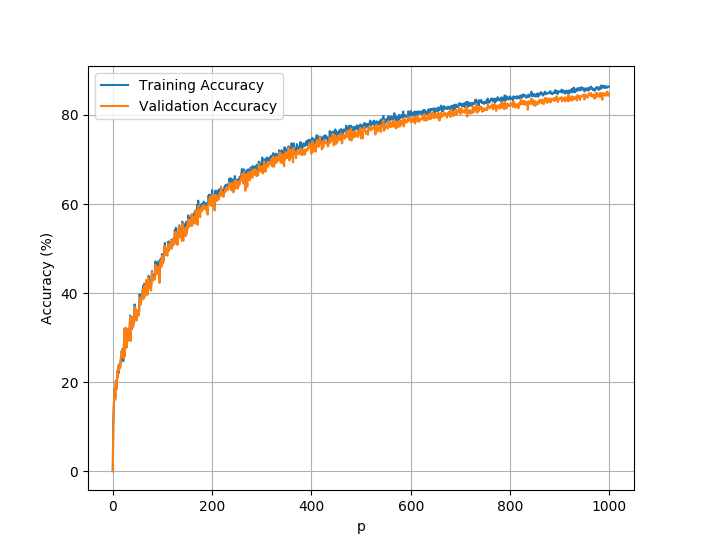
\includegraphics[width=4in]{CrossVal.png}

\item Instead of reporting just the classification test error, which is an unbiased estimate of the \emph{true} error, we would like to report a \emph{confidence interval} around the test error that contains the true error.
For any $\delta \in (0,1)$, it follows from Hoeffding's inequality that if $X_i$ for all $i=1,\dots,m$ are i.i.d. random variables with $X_i \in [a,b]$ and $\E[X_i] = \mu$, then with probability at least $1-\delta$ 
\begin{align*}
\P\left( \left| \left(\frac{1}{m} \sum_{i=1}^m X_i\right) - \mu \right| \geq \sqrt{\frac{\log(2/\delta)}{2m}} \right) \leq \delta
\end{align*}
We will use the above equation to construct a confidence interval around our true classification error since the test error is just the average of indicator variables taking values in $0$ or $1$ corresponding to the $i$th test example being classified correctly or not, respectively, where an error happens with probability $\mu$, the \emph{true} classification error. 

Let $\widehat{p}$ be the value of $p$ that approximately minimizes the validation error on the plot you just made and use $\widehat{W}^{\widehat{p}}$ to compute the classification test accuracy, which we will denote as $E_{test}$. 
Use Hoeffding's inequality, above, to compute a confidence interval that contains $\E[E_{test}]$ (i.e., the \emph{true} error) with probability at least $0.95$ (i.e., $\delta=0.05$).
Report $E_{test}$ and the confidence interval. 
\begin{lstlisting}[language=Python]
import numpy as np
import matplotlib.pyplot as plt
from mnist import MNIST
import random
import time

from numpy.core.multiarray import ndarray

X_train = []
X_test = []
labels_train = []
labels_test = []


def load_dataset():
    global X_train, X_test, labels_test, labels_train
    mndata = MNIST('./python-mnist/data/')
    X_train, labels_train = map(np.array, mndata.load_training())
    X_test, labels_test = map(np.array, mndata.load_testing())
    X_train = X_train/255.0
    X_test = X_test/255.0


def one_hot(inpt):
    output = np.zeros((inpt.size, 10))
    for i in range(len(inpt)):
        vec = np.zeros(10)
        for j in range(10):
            vec[j] = int(int(inpt[i]) == j)
            output[i] = vec
    return output


def train(X, y, lamb):
    w = np.linalg.solve(np.dot(np.transpose(X), X)+lamb*np.identity(X.shape[1]), np.dot(np.transpose(X), y))
    return w


def predict(w, x):
    y=np.dot(np.transpose(w), np.transpose(x))
    return np.argmax(y, axis=0)

def generateTransform(inpt, p, sigma):
    G = sigma*np.random.randn(inpt.shape[1], p)
    b = np.random.uniform(0, 2*np.pi, (p, 1))

    return G, b


def transform(inpt, G, b):
    out = np.transpose(np.cos(np.dot(np.transpose(G), np.transpose(inpt))+b))
    return out


def split(x, y, ylist, frac):
    index = random.sample(range(x.shape[0]), int(x.shape[0]*frac))
    xmajor = x[index]
    xminor = np.delete(x, index, 0)
    ymajor = y[index]
    yminor = np.delete(y, index, 0)
    listmajor = ylist[index]
    listminor = np.delete(ylist, index, 0)

    return xmajor, xminor, ymajor, yminor, listmajor, listminor


load_dataset()

y_train=one_hot(labels_train)
w = train(X_train, y_train, 10**-4)

print("No transformation")
print("Training Accuracy: "+str(sum(predict(w, X_train) == labels_train)/len(X_train)*100)+"%")
print("Testing Accuracy: "+str(sum(predict(w, X_test) == labels_test)/len(X_test)*100)+"%")

pmax=1*10**3
trainErr = np.zeros((pmax, 1))
valErr = np.zeros((pmax, 1))
for p in range(1, pmax):
    start=time.time()
    G, b= generateTransform(X_train, p, np.sqrt(0.1))
    transX = transform(X_train, G, b)
    trainX, valX, trainY, valY, trainList, valList = split(transX, y_train, labels_train, 0.8)
    w= train(trainX, trainY, 10**-4)
    trainErr[p] = sum(predict(w, trainX) == trainList) / len(trainX)*100
    valErr[p] = sum(predict(w, valX) == valList) / len(valX)*100
    end=time.time()
    print(str(round(p/pmax*100, 3))+"% Done")
    print(str(round((end-start)*(pmax-p),2))+" s left")


pOpt = np.argmax(valErr)
G, b = generateTransform(X_train, p, 0.01)
transX = transform(X_train, G, b)
trainX, valX, trainY, valY, trainList, valList = split(transX, y_train, labels_train, 0.8)
w = train(trainX, trainY, 10**-4)

print("With transformation")
print("Training Accuracy: "+str(sum(predict(w, trainX) == trainList)/len(trainX)*100)+"%")
print("Testing Accuracy: "+str(sum(predict(w, transform(X_test, G, b)) == labels_test)/len(X_test)*100)+"%")

plt.plot(trainErr)
plt.plot(valErr)
plt.grid()
plt.ylabel("Accuracy (%)")
plt.xlabel("p")
plt.legend(("Training Accuracy", "Validation Accuracy"))
plt.show()
\end{lstlisting}


\end{enumerate}

\end{document}
